\documentclass[tikz,border=3mm]{standalone}

\usepackage{pgfplots}

\pgfplotsset{compat=1.17}

\usepackage{xcolor}
\colorlet{myred}{red!80!black}
\colorlet{myblue}{blue!80!black}
\colorlet{mybluee}{myblue!80!black}

\begin{document}
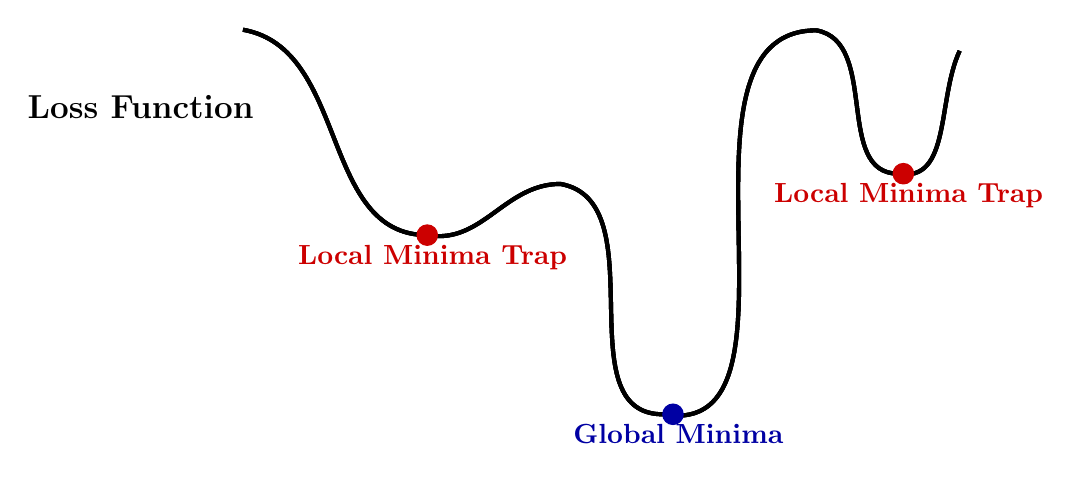
\begin{tikzpicture}[scale = 1.3]
  \coordinate (lkant) at (0,4.756);
  \coordinate (lmen) at (1.8, 2.75);
  \coordinate (lman) at (3.1, 3.25);
  \coordinate (bottom) at (4.1, 1);
  \coordinate (rman) at (5.6, 4.75);
  \coordinate (rmen) at (6.4, 3.35);
  \coordinate (rkant) at (7, 4.55);
  \coordinate (o) at (0,0);
  \coordinate (x) at (7,0);
  \coordinate (y) at (0,5);
  \coordinate (bottomm) at (4.2, 1);
  \coordinate (rmenn) at (6.45, 3.35);

  \draw [black, in=180, out=0, tension=.1, line width=1.5pt]
  (lkant)[out=-10] to (lmen) to (lman) to (bottom) to (rman) to (rmen)
  to [in=245](rkant);

  % \draw [<->] (y) -- node [rotate=90, above] {} (o) -> node [below] {} (x);

  \draw [black, in=180, out=0, tension=.1, line width=1.5pt]
  (lkant)[out=-10] to (lmen) to (lman) to (bottom) to (rman) to (rmen)
  to [in=245](rkant);
  \draw [black, in=180, out=0, tension=.1, line width=1.5pt]
  (lkant)[out=-10] to (lmen) to (lman) to (bottom) to (rman) to (rmen)
  to [in=245](rkant);

  \filldraw[color = mybluee] (bottomm) circle  (0.1) node [below,color=black] { \textbf{ \textcolor{mybluee}{Global Minima}}};
  \filldraw [color = myred] (lmen) circle (0.1) node [below,color=black] { \textbf{ \textcolor{myred}{Local Minima Trap}}};
  \filldraw [color = myred] (rmenn) circle (0.1) node [below,color=black] { \textbf{ \textcolor{myred}{Local Minima Trap}}};

  \node[draw=none, fill=none, text=black, inner sep=0pt] at (-1,4) {\large\textbf{Loss Function}};
\end{tikzpicture}
\end{document}